\documentclass{article}

\usepackage{fancyhdr}
\usepackage{extramarks}
\usepackage{amsmath}
\usepackage{amsthm}
\usepackage{amsfonts}
\usepackage{tikz}
\usepackage[plain]{algorithm}
\usepackage{algpseudocode}
\usepackage{xcolor}
\usepackage{enumitem}
\usepackage{amssymb}
\usepackage{todonotes}
\usepackage{mathtools}
\usepackage{wasysym}
\usepackage{cancel}
\usepackage{listings}

\usetikzlibrary{automata,positioning}

%
% Basic Document Settings
%

\definecolor{mygreen}{rgb}{0,0.6,0}
\definecolor{mygray}{rgb}{0.5,0.5,0.5}
\definecolor{mymauve}{rgb}{0.58,0,0.82}

\lstset{
  backgroundcolor=\color{white},   % choose the background color; you must add \usepackage{color} or \usepackage{xcolor}; should come as last argument
  basicstyle=\footnotesize,        % the size of the fonts that are used for the code
  breakatwhitespace=false,         % sets if automatic breaks should only happen at whitespace
  breaklines=true,                 % sets automatic line breaking
  captionpos=b,                    % sets the caption-position to bottom
  commentstyle=\color{mygreen},    % comment style
  deletekeywords={...},            % if you want to delete keywords from the given language
  escapeinside={\%*}{*)},          % if you want to add LaTeX within your code
  extendedchars=true,              % lets you use non-ASCII characters; for 8-bits encodings only, does not work with UTF-8
  frame=single,	                   % adds a frame around the code
  keepspaces=true,                 % keeps spaces in text, useful for keeping indentation of code (possibly needs columns=flexible)
  keywordstyle=\color{orange!90!black},       % keyword style
  language=Java,                 % the language of the code
  morekeywords={*,...},            % if you want to add more keywords to the set
  numbers=left,                    % where to put the line-numbers; possible values are (none, left, right)
  numbersep=5pt,                   % how far the line-numbers are from the code
  numberstyle=\tiny\color{mygray}, % the style that is used for the line-numbers
  rulecolor=\color{black},         % if not set, the frame-color may be changed on line-breaks within not-black text (e.g. comments (green here))
  showspaces=false,                % show spaces everywhere adding particular underscores; it overrides 'showstringspaces'
  showstringspaces=false,          % underline spaces within strings only
  showtabs=false,                  % show tabs within strings adding particular underscores
  stepnumber=1,                    % the step between two line-numbers. If it's 1, each line will be numbered
  stringstyle=\color{yellow!60!orange!80!black},     % string literal style
  tabsize=2,	                   % sets default tabsize to 2 spaces
  title=\lstname,                   % show the filename of files included with \lstinputlisting; also try caption instead of title
  keywords=[3]{self},
  keywordstyle=[3]{\color{orange!50!gray}},
  keywords=[4]{__init__, __lt__},
  keywordstyle=[4]{\color{orange!50!gray}},
  moredelim=**[is][\color{orange!90!black}]{@}{@}
}


\topmargin=-0.45in
\evensidemargin=0in
\oddsidemargin=0in
\textwidth=6.5in
\textheight=9.0in
\headsep=0.25in

\linespread{1.1}

\pagestyle{fancy}
\lhead{\hmwkAuthorName}
\chead{\hspace{2.5cm} \hmwkClass\ (\hmwkClassInstructor): \hmwkTitle}
\rhead{\firstxmark}
\lfoot{\lastxmark}
\cfoot{\thepage}

\renewcommand\headrulewidth{0.4pt}
\renewcommand\footrulewidth{0.4pt}

\setlength\parindent{0pt}

%
% Create Problem Sections
%

\newcommand{\enterProblemHeader}[1]{
    \nobreak\extramarks{}{Problem \arabic{#1} continued on next page\ldots}\nobreak{}
    \nobreak\extramarks{Problem \arabic{#1} (continued)}{Problem \arabic{#1} continued on next page\ldots}\nobreak{}
}

\newcommand{\exitProblemHeader}[1]{
    \nobreak\extramarks{Problem \arabic{#1} (continued)}{Problem \arabic{#1} continued on next page\ldots}\nobreak{}
    \stepcounter{#1}
    \nobreak\extramarks{Problem \arabic{#1}}{}\nobreak{}
}

\newcount\colveccount
\newcommand*\colvec[1]{
        \global\colveccount#1
        \begin{pmatrix}
        \colvecnext
}
\def\colvecnext#1{
        #1
        \global\advance\colveccount-1
        \ifnum\colveccount>0
                \\
                \expandafter\colvecnext
        \else
                \end{pmatrix}
        \fi
}

\setcounter{secnumdepth}{0}
\newcounter{partCounter}
\newcounter{homeworkProblemCounter}
\setcounter{homeworkProblemCounter}{1}
\nobreak\extramarks{Problem \arabic{homeworkProblemCounter}}{}\nobreak{}

%
% Homework Problem Environment
%
% This environment takes an optional argument. When given, it will adjust the
% problem counter. This is useful for when the problems given for your
% assignment aren't sequential. See the last 3 problems of this template for an
% example.
%
\newenvironment{homeworkProblem}[1][-1]{
    \ifnum#1>0
        \setcounter{homeworkProblemCounter}{#1}
    \fi
    \section{Problem \arabic{homeworkProblemCounter}}
    \setcounter{partCounter}{1}
    \enterProblemHeader{homeworkProblemCounter}
}{
    \exitProblemHeader{homeworkProblemCounter}
}

%
% Homework Details
%   - Title
%   - Due date
%   - Class
%   - Section/Time
%   - Instructor
%   - Author
%

\newcommand{\hmwkTitle}{Assignment 2}
\newcommand{\hmwkDueDate}{October 28, 2018}
\newcommand{\hmwkClass}{PF3}
\newcommand{\hmwkClassTime}{Spring Semester}
\newcommand{\hmwkClassInstructor}{Prof. Walter Binder }
\newcommand{\hmwkAuthorName}{\textbf{A. Romanelli}}

%
% Title Page
%

\title{
    \vspace{2in}
    \textmd{\textbf{\hmwkClass:\ \hmwkTitle}}\\
    \normalsize\vspace{0.1in}\small{Due\ on\ \hmwkDueDate\ at 8:30am}\\
    \vspace{0.1in}\large{\textit{\hmwkClassInstructor}}
    \vspace{3in}
}

\author{\hmwkAuthorName}
\date{}

\renewcommand{\part}[1]{\textbf{\large Part \Alph{partCounter}}\stepcounter{partCounter}\\}

%
% Various Helper Commands
%

% Useful for algorithms
\newcommand{\alg}[1]{\textsc{\bfseries \footnotesize #1}}

% For derivatives
\newcommand{\deriv}[1]{\frac{\mathrm{d}}{\mathrm{d}x} (#1)}

% For partial derivatives
\newcommand{\pderiv}[2]{\frac{\partial}{\partial #1} (#2)}

% Integral dx
\newcommand{\dx}{\mathrm{d}x}

% Alias for the Solution section header
\newcommand{\solution}{\textbf{\large Solution}}

% Probability commands: Expectation, Variance, Covariance, Bias
\newcommand{\E}{\mathrm{E}}
\newcommand{\Var}{\mathrm{Var}}
\newcommand{\Cov}{\mathrm{Cov}}
\newcommand{\Bias}{\mathrm{Bias}}

\begin{document}

\maketitle

\pagebreak

\begin{homeworkProblem}
	The entirety of this problem was done by writing the requested implementations. Please refer to the submitted source code files. The code for this particular exercise can be found in the following zip:
	\begin{center}
		\texttt{assignment2\_Romanelli\_Alessandro.zip}
	\end{center}
	Package \verb|exercise1| holds all the relevant source files.
\end{homeworkProblem}
\begin{homeworkProblem}
	\begin{enumerate}
		\item The current implementation violates the SRP because the \verb|AdPublisher| class lacks of functional cohesion. This means that it's quite difficult to identify a single well-defined task. Moreover, this class also violates the OCP principle, as it's not easily extendable and extending the functionality would mean to modify the already existing code.
		\item Here's the UML class diagram of revised design, which should be compliant to the OCP exploiting the \emph{Strategy Pattern}:
		\begin{figure}[h]
			\centering
			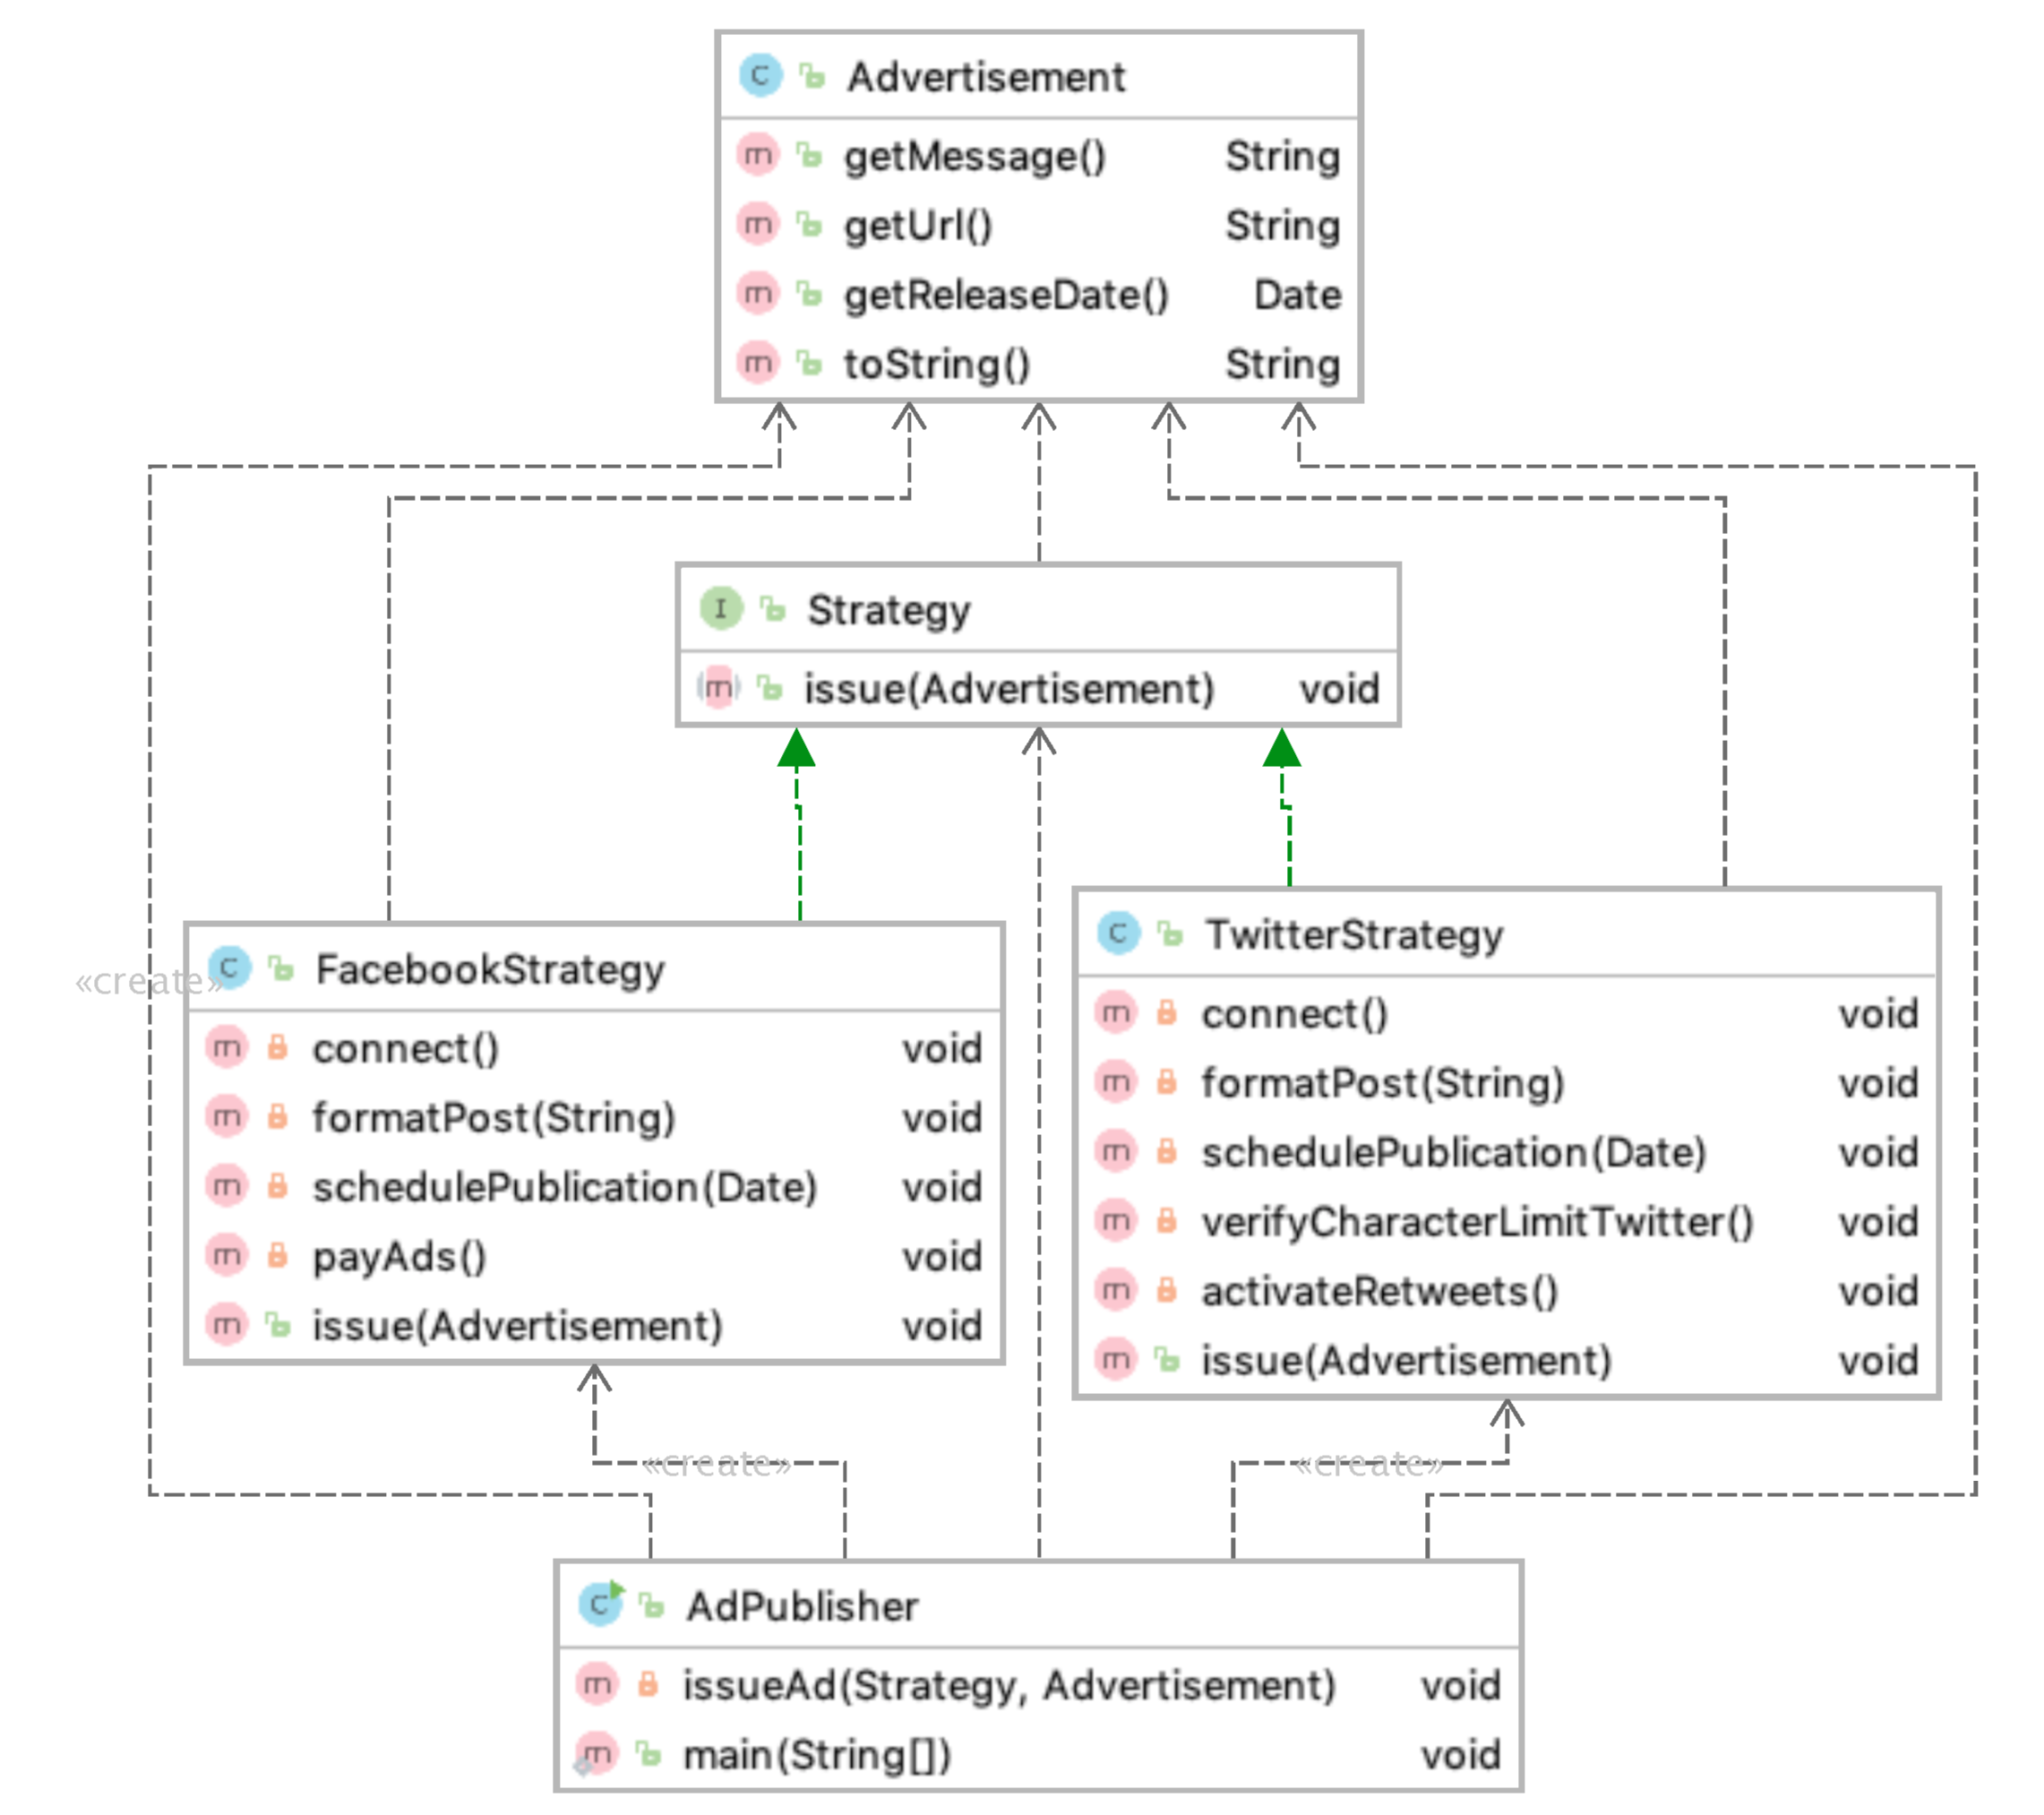
\includegraphics[width=0.80\textwidth]{uml_graph}
			\caption{UML Class Diagram}
		\end{figure} \\
		This class diagram is not strictly compliant to the SRP: each Strategy handles several aspects of how an ad is issued. However, this was done to avoid the creation of too many classes, which would have caused the loss of the OCP.
		\item[3.| 4.] The points of this problem requiring the actual implementations can be found in the zip:
			\begin{center}\texttt{assignment2\_Romanelli\_Alessandro.zip}
			\end{center}
			Refer to the source files within package \verb|exercise2|
		\item[5.] In order to illustrate why the Strategy pattern is so effective we can take a look at how I implemented the \verb|InstagramStrategy|. The implementation of said Strategy is based on implementing the interface Strategy, which provides the core functionality. Being independent from the other Strategies, I was able to implement Instagram-specific methods with ease and that didn't affect the functionality of the other strategies. To then make use of the new strategy within my test program, because of the intrinsic interchangeability, I only needed to create a \verb|new InstagramStrategy()| and utilise it as any other implementation of a \verb|Strategy| interface.
	\end{enumerate}
\end{homeworkProblem}
\section{Bonus Problem}
	Refer to the attached source code files for this exercise which can be found in the following zip: 
	\begin{center}
		\texttt{assignment2\_Romanelli\_Alessandro.zip}
	\end{center}
	The relevant files for this problem can be found in the package \verb|exercise3|.
\end{document}
